%:Clase del documento
\documentclass[fontsize=10pt, Myfinal=true, twoside, numbers=noenddot]{scrbook}
%Minion=true, English=true, Myfinal=true

%:Paquete de estilos propuesto
\usepackage{cabeceras/libroETSI}

%:Paquete específico para cargar tikz (y sus librerías) y pgfplots
\usepackage{cabeceras/dtsc-creafig}

%:Paquete para notaciones específicas
\usepackage{cabeceras/notacion}

%:Paquete para incorporar aspectos concretos de la edición
\usepackage{cabeceras/edicionPFC}


%:Estas líneas de código son INNECESARIAS excepto para mostrar determinadas características en este manual. Pueden eliminarse o comentarse sin ningún problema.
%Se usan para compilar el capítulo estilolibroetsi.tex
\usepackage[final]{showexpl}
\lstset{explpreset={frame=none,rframe={}, numbers=none,numbersep=3pt, columns=flexible,language={[LaTeX]TeX},basicstyle=\ttfamily,keywordstyle=\color{blue}}}%numberstyle=\tiny,

%:Para modificar fácilmente la fuente del texto.
\makeatletter
\ifdtsc@Minion % Queremos utilizar la fuente Minion y lo hemos declarado al principio
	\ifluatex
		\setmainfont[Renderer=Basic, Ligatures=TeX,	% Fuente del texto 
		Scale=1.01,
		]{Minion Pro}
   		% En este caso conviene modificar ligeramente el tamaño de las fuentes matemáticas
		\DeclareMathSizes{10}{10.5}{7.35}{5.25}
		\DeclareMathSizes{10.95}{11.55}{8.08}{5.77}
		\DeclareMathSizes{12}{12.6}{8.82}{6.3}
%		\setmainfont[Renderer=Basic, Ligatures=TeX,	% Fuente del texto 
%		]{Adobe Garamond Pro}
%		\setmainfont[Renderer=Basic, Ligatures=TeX,	% Fuente del texto 
%		]{Palatino LT Std}
	\fi
\else
	\ifluatex
		% Para utilizar la fuente Times New Roman, o alguna otra que se tenga instalada
		\setmainfont[Renderer=Basic, Ligatures=TeX,	% Fuente del texto 
		Scale=1.0,
		]{Times New Roman}
	\else
		\usepackage{tgtermes} 	%clone of Times
		%\usepackage[default]{droidserif}
		%\usepackage{anttor} 	
	\fi
\fi
\makeatother

\usepackage[
    backend=biber,
    sorting=none, 
    %style=authoryear-icomp,
    %sortlocale=de_DE,
    %natbib=true,
    %url=false, 
    %doi=true,
    %eprint=false
]{biblatex}
\defbibheading{etsi}[]{%
        \chapter*{Bibliografía}%
        \chaptermark{Bibliografía} 
        \markboth{#1}{#1}}
\addbibresource{bibliografia.bib}

% Ejemplo de Glosario
\newacronym[type=main]{ETSI}{ETSI}{Escuela Técnica Superior de Ingeniería}
\newacronym[type=main]{US}{US}{Universidad de Sevilla}
\newacronym[type=main]{DMC}{DMC}{Canal Discreto sin Memoria}


\makeindex
\makeglossaries %Si no se quiere el glosario, comentar esta línea.

% Formato A4
\geometry
{paperheight=297mm,%
paperwidth=210mm,%
top=25mm,%
headsep=8.5mm,%
includefoot, 
textheight=240mm, 
textwidth=150mm, 
bindingoffset=0mm, 
twoside}

\usepackage[a4,center]{crop}%para poner las cruces de esquina de página, poner la opción cross

%:Esquema de numeración por defecto
\setenumerate[1]{label=\normalfont\bfseries{\arabic*.}, leftmargin=*, labelindent=\parindent}
\setenumerate[2]{label=\normalfont\bfseries{\alph*}), leftmargin=*}
\setenumerate[3]{label=\normalfont\bfseries{\roman*.}, leftmargin=*}
\setlist{itemsep=.1em}
\setlength{\parindent}{1.0 em}

\setcounter{tocdepth}{4}						% El nivel hasta el que se muestra el índice 

\usepackage{morewrites}
\usepackage[outputdir=build]{minted}
\setminted{fontsize=\footnotesize,linenos,breaklines,mathescape}
\usepackage[minted]{tcolorbox}
\tcbuselibrary{breakable,skins}

\newtcolorbox[auto counter,number within=chapter,list inside={qst}]{codigo}[2][]{,enhanced,breakable, left=1cm,colback=black!5!white,colframe=blue!0!black,fonttitle=\bfseries, title=Código ~\thetcbcounter: #2,#1}
\usepackage{adjustbox}
\usepackage{tikz-3dplot}
%\usepackage{subcaption}
\setcounter{secnumdepth}{40}

\usepackage{gensymb}

\usepackage{pdflscape}
\usepackage{multirow}
\usepackage{placeins}

\makeatletter
\providecommand\add@text{}
\newcommand\tagaddtext[1]{%
     \gdef\add@text{#1\gdef\add@text{}}}% 
     \renewcommand\tagform@[1]{%
          \maketag@@@{\llap{\add@text\quad}(\ignorespaces#1\unskip\@@italiccorr)}%
     }
\makeatother

\begin{document}
%:Para incluir toda la referencia bibliográfica aunque no se cite, descomente la siguiente línea
%\nocite{*}


%PORTADA
%ver edicionPFC.sty para modificaciones
%\mbox{pendiente}
%:Para crear la portada y la portada interior (pagina titular)
\titulo{Posicionamiento de un UAV Mediante los \mbox{Marcadores} Visuales Aruco y el \mbox{Estimador} de Estados de PX4} %\mbox evita que se divida una palabra al cambiar de línea
\autor{Isidro Jesús Arias Sánchez}
\director{Manuel Vargas Villanueva}
\titulodirector{Profesor Titular}

\departamento{Dpto. de Ingeniería de Sistemas y Automática}
\centro{Escuela Técnica Superior de Ingeniería}
\universidad{Universidad de Sevilla}
\titulacion{Ingeniería Electrónica, Robótica y Automática}
\fecha{2020}
\nombretrabajo{Trabajo de Fin de Master} %Trabajo Fin de Grado, Proyecto fin de Máster,....

\hypersetup
	{
 	linkcolor=black, %Tocar para poner color en enlaces
	pdfauthor={\elautor},
	pdftitle={\nombretrabajo,\eltitulo}, 
	pdfkeywords={Latex, edición, formato de texto}	
	 }

%\portadaPFC{figuras/LogoUS.pdf}{figuras/LogoTSC.pdf} %logo de la Universidad y logo del departamento, si lo hubiera. Para cambiar el pie de página con los logos, debe editarse el fichero ediciónPFC.sty
\portadaPFC{figuras/LogoUS.pdf} %logo de la Universidad y logo del departamento, si lo hubiera. Para cambiar el pie de página con los logos, debe editarse el fichero ediciónPFC.sty

%Fin Portada

\frontmatter
\pagenumbering{Roman} %Pone la numeración en mayúscula (En español parece que es obligatorio)

%\include{dedicatoria/dedicatoria}
%% !TEX root =../LibroTipoETSI.tex
\chapter*{Agradecimientos}
%\pagestyle{especial}
\pagestyle{empty}
%\chaptermark{Agradecimientos}
\phantomsection
%\addcontentsline{toc}{listasf}{Agradecimientos}
%\vspace{1cm}
%{\huge{Agradecimientos}}
%\vspace{1cm}

\lettrine[lraise=-0.1, lines=2, loversize=0.25]{E}{stos} 4 años han sido mejores gracias al apoyo de algunas personas. Especialmente quiero agradecérselo a mis padres, Mercedes y José, a mi tía Antonia, a mi abuela Mercedes, a mi hermano Héctor, a Candi, mi novia, a mis amigos de Sevilla, Ángel, Carlos, David, Fernando, Jorge y Samuel, a los de Cádiz, Daniel, Juan Luís, Javier Mena, Javier Sanz, Pepe y Pedro, y por último y no menos importante, a mi tutores Manuel Vargas y Manuel Gil, y al resto de los profesores que me han sabido enseñar y de los que tanto he aprendido. Gracias a todos. 

{\flushleft{\hfill \emph{Isidro Arias Sánchez}}}%
\vspace{-.3cm}
%{\flushleft{\hfill \emph{Estudiante del Grado en Ingenieria Electrónica, Robótica y Mecatrónica}}}%
{\flushleft{\hfill \emph{Sevilla, 2019}}}%


\def\entregar{1}

% !TEX root =../LibroTipoETSI.tex
\chapter*{Resumen}
\pagestyle{especial}
\chaptermark{Resumen}
\phantomsection
\addcontentsline{toc}{listasf}{Resumen}

%\lettrine[lraise=-0.1, lines=2, loversize=0.2]{E}{n} este proyecto  se va a desarrollar el  estudio de  un vehículo aéreo no tripulado que tiene dos hélices o rotores orientables, denominado tiltrotor, del ingles \textit{tilt} que significa inclinar.

{\color{red} [Pendiente]}



\chapter*{Abstract}
\pagestyle{especial}
\chaptermark{Abstract}
\phantomsection
\addcontentsline{toc}{listasf}{Abstract}

%\lettrine[lraise=-0.1, lines=2, loversize=0.2]{T}{he} basis of this work is to contribute to the study of a convertible aerial vehicle in which the rotors, being tiltable, operate with the advantages of two different aircraft models, one of the helicopter type that gives it high maneuverability, and one of the airplane type that allows traveling long distances.

{\color{red} [Pendiente]}

 

% Índice abreviado 
% El índice abreviado se incluye también en algunos libros, con menor detalle que el completo. Descomentar las siguientes líneas.
\cleardoublepage
\phantomsection
\addcontentsline{toc}{listasf}{Índice Abreviado}
\pagestyle{especial}
\shorttoc{Índice Abreviado}{1}

%Índice normal, el completo
\cleardoublepage
\phantomsection
\pagestyle{especial}
\tableofcontents


\chapter*{\notationname}
\pagestyle{especial}
\chaptermark{\notationname}
\phantomsection
\addcontentsline{toc}{listasf}{\notationname}
\begin{longtable}{p{3cm}p{8.5cm}}
%TODO: Actualizar la notación de este trabajo
$\bm{P}$ & Posición del vehículo en ejes inerciales  \\
$\bm{V}$ & Velocidad del vehículo en ejes inerciales \\
$\bm{T}$ & Empuje aplicado en ejes cuerpo \\
$\bm{T_{rot}}$ & Empuje aplicado en ejes inerciales \\
$\theta$ &  Inclinación del quadrotor \\
$\bm{\tau}$ &  Par aplicado al quadrotor \\
$\omega$ & Medida del giróscopo \\
$\bm{a}$ & Medida del acelerómetro \\
$R^{UAV\rightarrow C\acute{a}mara}$  & Orientación del marcador vista desde el vehículo\\
$\bm{X}$ &  Vector de estados \\
\end{longtable}
\newpage

\chapter*{Acrónimos}
\pagestyle{especial}
\chaptermark{Acrónimos}
\phantomsection
\addcontentsline{toc}{listasf}{Acrónimos}
\begin{longtable}{p{3cm}p{8.5cm}}
$UAV$ & Vehículo aéreo no tripulado\\
$GCS$ & Estación de control terrestre \\
$NED$ & Ejes norte, este y abajo \\
\end{longtable}
\newpage

 %No incluir si no se quiere, comentándolo

%%:Empieza el contenido del libro
\mainmatter

%:Página por defecto
\pagestyle{esitscCD}
\hypersetup { linkcolor=blue, } 

% !TEX root =../LibroTipoETSI.tex
%El anterior comando permite compilar este documento llamando al documento raíz
\chapter{Introducción}\label{chp-01}
\epigraph{All models are wrong, but some are useful}{George Box, 1976}

\lettrine[lraise=-0.1, lines=2, loversize=0.2]{E}{l} interés en los vehículos aéreos no tripulados UAV (\textit{Unmanned Aerial Vehicle}) está en aumento. Dos grandes sectores en el mercado de los UAVs son el de consumo, como aquellos que se usan con fines de ocio, y el comercial, como los que son usados en los negocios o instituciones para realizar algún tipo trabajo. 
Un ejemplo de su aplicación se puede ver en una prueba piloto \cite{telefonica} que consiste en utilizar las torres de comunicaciones para albergar un UAV que se dirige de forma autónoma hasta la zona de un posible incendio, si recibe un aviso de sensores infrarrojos situados en al misma torre de comunicaciones.
\begin{figure}
   %\centering
   \includegraphics[width=0.3\textwidth]{introduccion/drone-incendio.jpg}\ 
   \caption{Prueba piloto de UAV antiincendios. Fuente \cite{telefonica} }
   \label{fig:telefonica}
\end{figure}

Este último sector es el que se  espera que experimente un mayor aumento y se predice que su tamaño se triplique en el año 2023 \cite{mercado-drones}.
Su crecimiento se ve limitado por diversos factores entre los que destacan las regulaciones, como la necesidad de estar dentro del alcance visual del piloto, o la autonomía de las baterías. Esto último es más notorio en aquellos vehículos de ala rotativa como los helicópteros o quadrotors, ya que son mucho menos eficientes que los de ala fija como los aeroplanos. Sin embargo, tienen mayor maniobrabilidad que estos últimos puesto que, entre otras cosas, son capaces del despegue y aterrizaje en vertical. 

Dadas las ventajas de cada uno de estos tipos nace la idea de \textit{VTOL}, que son los aviones con capacidad de despegue vertical. Un caso de ellos son los tiltrotors, que son aquellos que poseen rotores (también llamados proprotores) que se inclinan. 
En \cite{tiltrotor-review} se hace una recopilación de los estudios sobre diferentes técnicas de control de estos vehículos, tanto de 2, 3 o 4 rotores. Para el caso de 2 rotores, en \cite{tiltrotor-control} y  \cite{tiltrotor-control2} se proponen distintos controladores.  


En este trabajo se diseñará un controlador para el modo helicóptero de un tiltrotor y se implementará en un autopiloto de código abierto llamado \textit{PX4}. Este es un proyecto comenzado en 2009 por la \textit{Escuela Politécnica Federal de Zúrich} (ETH) que ofrece todo el software necesario para hacer que los vehículos aéreos, acuáticos o terrestres naveguen de forma autónoma. 

~\cite{windup}

\endinput

% !TEX root =../main.tex
\chapter{Estimador PX4}\label{chp-01}

\lettrine[lraise=-0.1, lines=2, loversize=0.2]{E}{n} muchas ocasiones se tienen sensores con un retraso y una frecuencia de actualización muy diferentes entre ellos, por ejemplo una IMU es mucho más rápida que el procesamiento de la imagen de una cámara. PX4 lo soluciona añadiendo más elementos a la estructura original de un estimador de estados. Uno de los elementos es un \textit{Filtro de Kalman Extendido} (EKF). Este no usa las medidas más nuevas que le llegan, si no que las almacena y utiliza las que llegaron hace un determinado tiempo. Corriendo en paralelo pero a una frecuencia mayor, existe un estimador llamado \textit{Filtro de Salida}, el cual sí que utiliza la última medida del acelerómetro y del giróscopo. 

\section{Ejemplo}
Supongamos que se tiene un sistema que se mueve en el espacio del que se quiere conocer sus estados, en concreto, su posición, su velocidad y su ángulo. Para este objetivo se disponen de sensores que son: acelerómetro, giróscopo, GNSS y posición por visión. Cada uno de ellos tiene diferentes propiedades en cuanto a retraso, ruido, etc. que se muestran en la siguiente tabla. Se puede notar que la posición por visión es una fuente muy precisa de posición, pero sin embargo tiene un gran retraso desde que se toma la imagen hasta que se procesa, como suele suceder en la práctica. 
\begin{tabular}{|c|c|c|}
Sensor			& Retraso (ms) 	& Ruido 	\\ \hline 
acelerómetro 		& 0 		& 	      	\\ 
giróscopo 		& 0 		& 	      	\\ 
GNSS      		& 		& 	      	\\ % eliminar? 
Posición por visión 	& 30 		& 0.03 	
% Flujo óptico?
\end{tabular}

% EKF

En el primera ejecución del estimador, después de inicializar los estados, se toma una medida de la IMU (acelerómetro y giróscopo). El EKF todavía no la utiliza, si no que la guarda en su buffer. Conforme llegan nuevas medidas, las que ya estaban en el buffer se van desplazando hacia la derecha, hasta que llegan a la última celda y entonces son usadas por el EKF para estimar los estados. Estos estados y las medidas utilizadas para estimarlos se refieren al \textit{horizonte de tiempo retrasado}. 

% llega medida de visión
Pasan algunos ciclos más hasta que en el instante 40ms llega la primera medida de la visión, pero esta no se coloca junto con las medidas más recientes de la IMU, si no que se lleva directamenta a la última celda. En esta se encuentran también las medidas de la IMU tomadas en el instante 10ms, es decir hace 30 ms que coincide con el retraso que tiene la posición visual con respecto a la IMU. De esta manera se agrupan las medidas que se refieren al mismo instante físico, es decir, el instante en el que llegaron compensandose su retraso. 
\\
\includegraphics[width=\textwidth]{estimador_px4/tikz/ekf_output}


% Filtro de salida

De forma paralela se ejecuta el \textit{filtro de salida} que solamente utiliza las medidas de la IMU, en este caso las que se generan más recientemente.
Los estados de este último filtro, la posición, velocidad y orientación,  se han estado guardando en el \textit{buffer de salida}.  
De este buffer se cogen los estados más antiguos y se compara con los estados generados por EKF. Su diferencia se multiplica por una ganancia se le suma a todos los elementos del buffer de salida.  

\subsection{Detalles de implementación}
\begin{itemize}
\item La ganancia que multiplica la diferencia entre el filtro de salida y el EKF y que sirve para corregir los estados, se calcula de manera el sistema controlado tenga un factor de amortiguamiento de 0.7
\begin{equation}
K_p=\frac{0.5}{Retraso}
\end{equation} 
{\color{red} Buscar la deducción hasta esta expresión}
\end{itemize}
\section{EKF para modelo bidimensional}
Se va aplicar a un quadrotor en 2 dimensiones, pero el modelo al no ser dinámico, se podria aplicar a cualquier otro móvil.

Estados:
\begin{align}
X = 
\begin{bmatrix} 
x \\ y \\ V_x \\ V_y \\ \theta
\end{bmatrix}
\end{align}

Modelo de predicción (modelo cinemático, no dinámico):
\begin{align}
\begin{bmatrix} 
x \\ y 
\end{bmatrix}_{k+1}
=
\begin{bmatrix} 
x \\ y 
\end{bmatrix}_k
+
\begin{bmatrix} 
V_x \\ V_y 
\end{bmatrix}_k
\Delta t
\end{align}

\begin{align}
\begin{bmatrix} 
V_x \\ V_y 
\end{bmatrix}_{k+1}
=
\begin{bmatrix} 
V_x \\ V_y 
\end{bmatrix}_k + 
\Delta t
\begin{bmatrix} 
\cos{\theta} & \sin{\theta} \\ -\sin{\theta} & \cos{\theta}
\end{bmatrix}
\bm{a} +  
\begin{bmatrix} 
0 \\ - m\ g 
\end{bmatrix}\Delta t
\end{align}

\begin{align}
\theta_{k+1} = \theta_k + \Delta t \omega
\end{align}


Jacobiano del modelo de predicción:
\begin{align}
F = 
\begin{bmatrix} 
%x/X
1 	&0	&\Delta t	&0		&0\\
%y/X
0 	&1	&0		&\Delta t	&0\\
%Vx/X
0 	&0	&1		&0		&\Delta t\left(-a_x\sin{\theta} + a_y\cos{\theta}\right) \\
%Vy/X
0 	&0	&0		&1		&\Delta t\left(-a_x\cos{\theta} - a_y\sin{\theta}\right) \\
%theta/X
0 	&0	&0		&0		&1
\end{bmatrix}
\end{align}

Jacobiano del acelerómetro y el giróscopo
\begin{align}
G = 
\begin{bmatrix} 
%x/a,w
0 			&0			&0\\
%y/a,w
0 			&0			&0\\
%Vx/a,w
\Delta t \cos{\theta} 	&\Delta t \sin{\theta}	&0\\
%Vy/a,w
-\Delta t \sin{\theta} 	&\Delta t \cos{\theta}	&0\\
%theta/a,w
0 			&0			&1		
\end{bmatrix}
\end{align}

Matriz de covarianzas de la predicción:
\begin{align}
Q = 
G
\begin{bmatrix} 
\sigma^2_a 	& 0 		& 0\\
0 		& \sigma^2_a 	& 0\\
0 		& 0 		& \sigma^2_\omega\\
\end{bmatrix}
G^T
\end{align}


\endinput

% !TEX root =../main.tex
\chapter{Posicionamiento mediante marcadores visuales}\label{chp-01}


%%% Figuras %%%%
\def\figFlow{
%TODO: añadir conexión con autopiloto y pequeña descripción interna
%TODO: añadir imagen de cámara en su bloque 
\begin{figure}
\includegraphics[width=\textwidth]{posicionamiento_marcadores/tikz/diagrama_flujo}
\caption{A la izquierda: diagrama de flujo del programa que se corre en el ordenador embebido, a la derecha: algunas de las tareas del autopiloto}
\label{fig:flow}
\end{figure}
}

\def\figEjes{
\begin{figure}
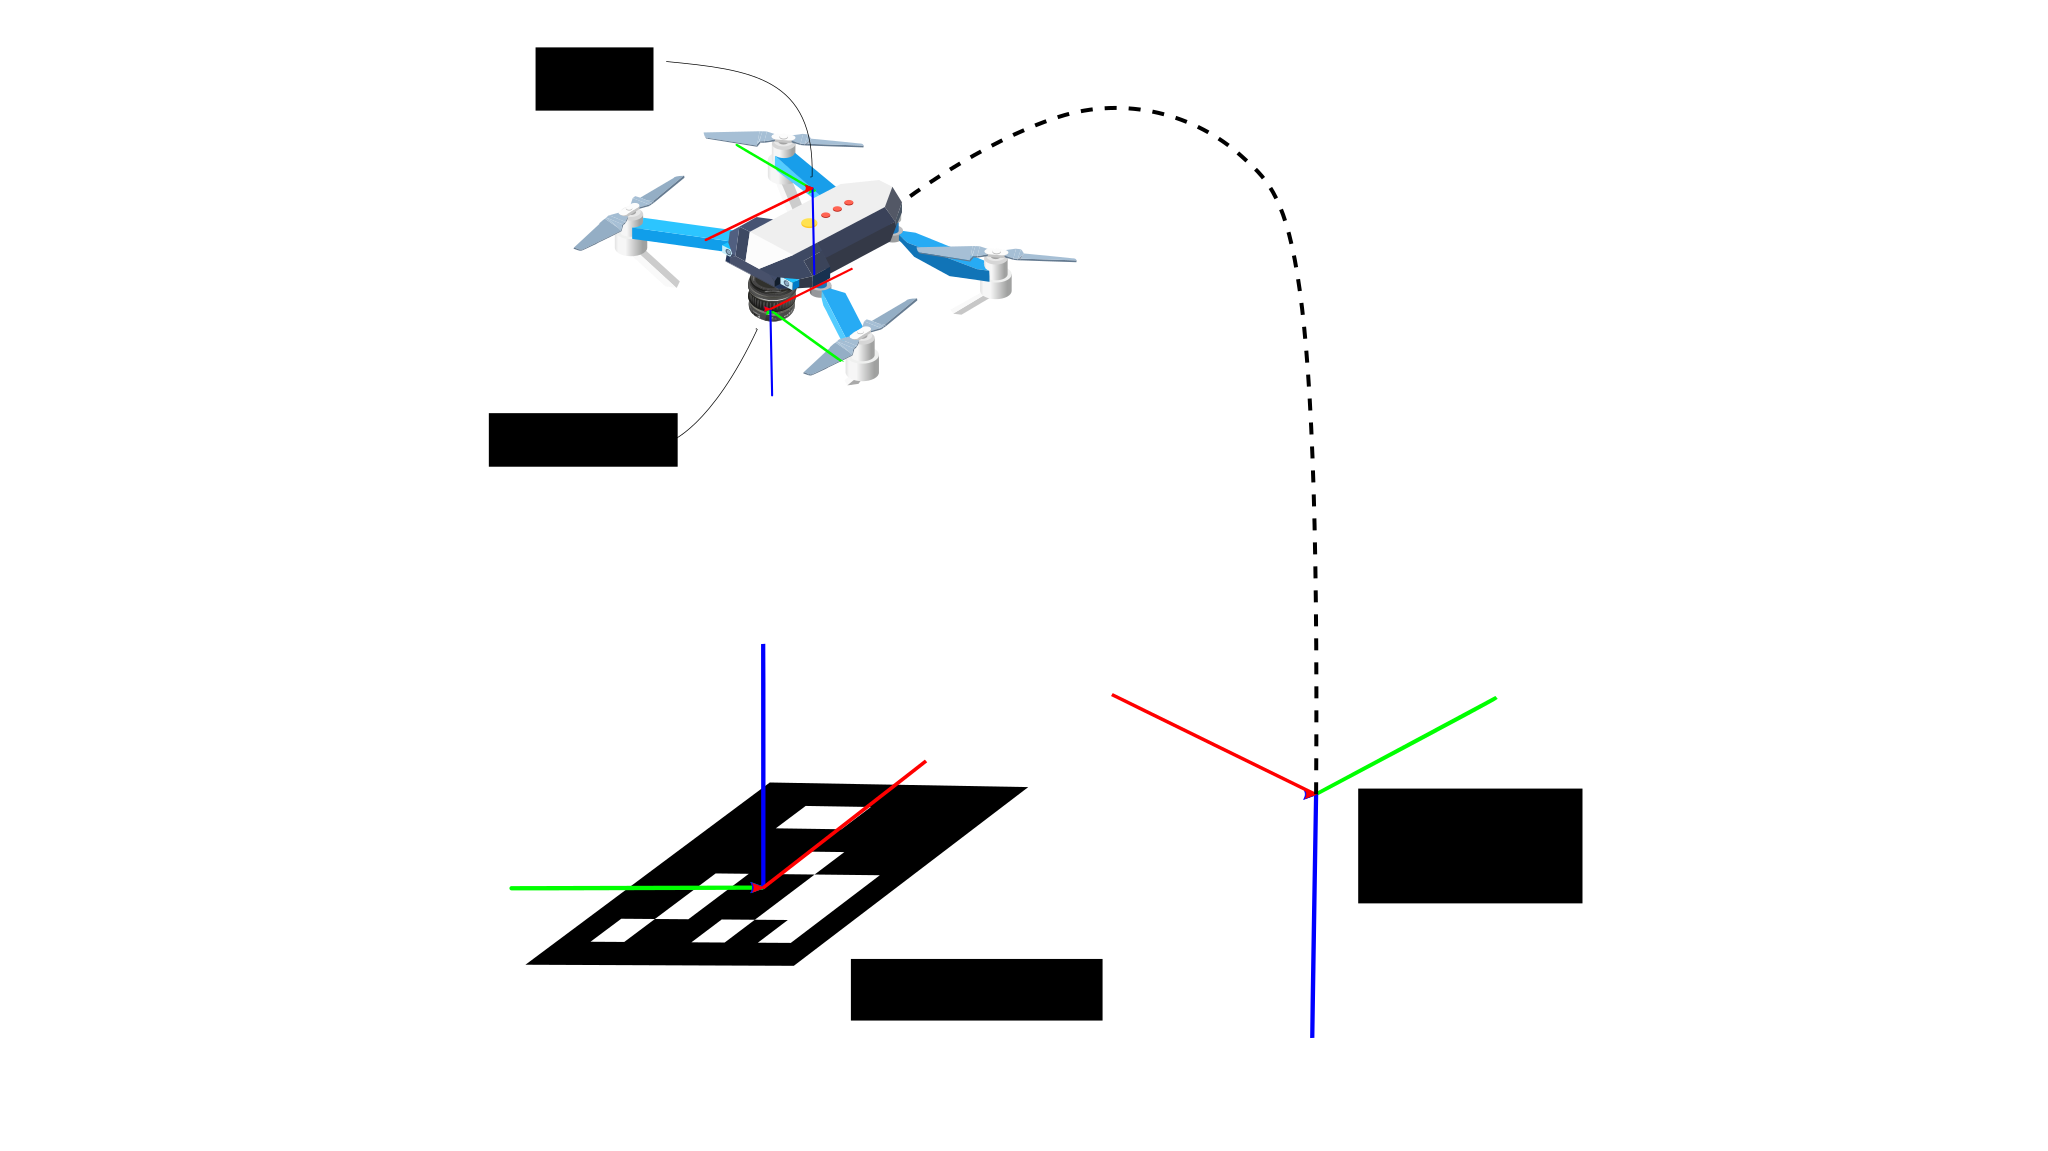
\includegraphics[width=\textwidth]{posicionamiento_marcadores/ejes}
\caption{Sistemas de referencia presentes en el problema}
\label{fig:ejes}
\end{figure}
}


% Más concretamente la precisión que se busca es centimétrica, pensando en coger un objeto metálico de manera autónoma con un imán colgando del UAV
\lettrine[lraise=-0.1, lines=2, loversize=0.2]{C}{onseguir} con precisión la posición de un vehículo aéreo no tripulado es bastante deseable. En la introducción se comentó aplicaciones como la manipulación de objetos o la navegación cerca de obstáculos. En este cápitulo se explica que para conseguirlo se ha construido un quadrotor con los componentes necesarios para detectar un marcador visual y cómo se ha programado un ordenador embebido en el quadrotor para que procese dicho marcador. 

De manera resumida, el funcionamiento es el siguiente:
- Se ha colocado un una cámara en la parte inferior del quadrotor, conectada a un ordenador embebido que procesa las imágenes tomadas
- En el suelo se coloca un marcador impreso que es detectado por la cámara
- Este le envía al autopiloto la posición y orientación del UAV con respecto a los ejes de coordenadas del del marcador 
- El autopiloto lo recibe, lo fusiona en su estimador de estados
- El estimador genera una posición estimada que alimenta al controlador de posición
- El controlador de posición toma esta medida y sigue la referencia. Esta última puede venir o bien del mando (consignas de movimiento en ejes inerciales) o del ordenador embebido el cual le indique una trayectoria.

Nótese que el controlador de posición también se podría haber ubicado en el ordenador embebido, generando consignas de aceleración en ejes cuerpo en función de los errores de posición en ejes cuerpo. La desventaja de esto es que se no se utilizan los demás sensores para el posicionamiento, por ejemplo si en un instante falta la medida de la visión, el autopiloto podría tomar otras como el acelerómetro, el GPS, el flujo óptico... 

\section{Mi programa}

\figFlow

%\begin{figure}
%\includegraphics[width=\textwidth]{posicionamiento_marcadores/pasosAruco}
%\caption{Pasos del proceso de detección de marcadores}
%\label{fig:pasosAruco}
%\end{figure}

- Inicialización: 
- Recoger imagen de la cámara: Este podría llegar a ser muy lento si no se escoge una interfaz con la cámara adecuada, por ejemplo USB. En este caso se ha escogido CSI que lleva la imagen directamente a la GPU y esta la lleva mediante DMA a la RAM. Todo ello sin consumir tiempo de CPU permitiendo que esta haga en paralelo otras operaciones como el procesamiento de imagen.
- Detectar marcadores: El objetivo es ubicar los marcadores de la imagen y extraer su identificador.  Este proceso está explicado en \cite{aruco2014}, pero lo que se va a aportar aquí es una referencia directa al código de la librería aruco y a algunas funciones implementadas. 
	- 1. El primer paso es la extración de bordes a partir de la imagen convertida a blanco y negro. 
	- 2. A partir de la imagen binaria del paso anterior, se extraen los contornos usando en \textit{\_findMarkerContours()} la función de OpenCV  \textit{}
	- 3. Se realiza una aproximación poligonal y se quedan aquellos que solo estén compuestos por 4 puntos. 
- Estimación de la posición
	La estimación de la posición y la orientación se realiza tomando las esquinas de un marcador obtenido en el paso anterior.  
- Inversión de posición y orientación 
	Como se ve en la figura \ref{fig:ejes} hay varios sistemas de referencia que entran en juego y hay que tenerlos presente para tranformar desde lo que aporta la detección de marcadores hasta lo que necesita el autopiloto. En el paso anterior, la orientación y posición que se obtiene es la del \textbf{marcador con respecto a la cámara}, es decir se obtiene $R^{Marcador\rightarrow C\acute{a}mara}$ y $p^{Marcador\rightarrow C\acute{a}mara}$. En el código \ref{cod:inver} se puede ver que una vez obtenida dicha matriz de rotación esta se invierte o trasnpone para conseguir la orientación de la cámara vista desde el sistema de referencia del marcador. Dicha matriz se utiliza para expresar la posición del marcador en unos ejes rotados centrados en la cámara y paralelos a los ejes del marcador. Esta posición simplemente se niega para obtener la posición de la cámara vista desde el marcador $p^{C\acute{a}mara\rightarrow Marcador}$ que es la que se le envía al autopiloto. En cuanto a la orientación, como se ve en la figura, los ejes de la cámara y los del UAV están rotados 180\textdegree con respecto al eje z. Conociendo esto se obtiene la orientación del UAV visto desde el marcador:

	\begin{equation}
	R^{Marcador\rightarrow UAV}=\left( R^{C\acute{a}mara\rightarrow Marcador}\ R^{UAV\rightarrow C\acute{a}mara} \right)^T
	\end{equation}

	\figEjes

	\begin{codigo}{Inversión de la posición y orientación ubicada en mi archivo \textit{marker\_vison.h}}
	\label{cod:inver}
	\inputminted{c++}{posicionamiento_marcadores/cod_inver.cpp}
	\end{codigo} 

	% TODO: explicar rotación en ángulos de euler
	
- Envio al autopiloto 
	La orientación y la posición son enviadas a autopiloto a través del protocolo \textit{Mavlink}
	Una vez que las recive, este calcula la rotación entre su orientación expresada en ejes NED y su orientación expresada en el sistema de referencia de la visión, que en este caso es el del marcador. Como se puede ver en el código \ref{cod:invPX4} esta rotación se le aplica a la posición de la visión. El final la posición que utiliza PX4 para fusionar es la del UAV expresado en unos ejes centrados en el marcador y paralelos a los ejes NED. Que tengan está orientación es importante, que el EKF en su fase de predicción, utilizando el acelerómetro y la orientación estimada, expresa su posición en ejes NED.

	\begin{codigo}{Rotación en PX4 de la posición suministrada por la visión}
	\label{cod:invPX4}
	En el archivo \textit{ekf\_helper.cpp}:
	\begin{minted}[firstnumber=1460]{c++}
		const Quatf q_error((_state.quat_nominal * _ev_sample_delayed.quat.inversed()).normalized());
		_R_ev_to_ekf = Dcmf(q_error);
	\end{minted}
	En el archivo \textit{control.cpp}:
	\begin{minted}[firstnumber=273]{c++}
		ev_pos_meas = _R_ev_to_ekf * ev_pos_meas;
		ev_pos_var = _R_ev_to_ekf * ev_pos_var * _R_ev_to_ekf.transpose();
	\end{minted}
	\end{codigo} 



\section{Hardware}
Para elegir los componentes se ha tenido en cuenta que no estén discontinuados, para comprar posibles recambios, que estén ampliamente probados, y la rapidez de llegada ya que todos llegan por paquetería, y que en la medida de lo posible estuvieran liberados tanto su software como su hardware. 

\begin{itemize}
\item Raspberry pi 4 Model B. 4 GB de RAM. 
\item Raspberry Pi Camera Module v2. Campo de visión horizontal de 62 grados, capaz de grabar vídeo con resolución de 1640x1232 a 40fps.
\item Cama amortiguadora para el autopiloto.
\item Cuav V5+. Autopiloto corriendo PX4. Esquemáticos publicados en \href{https://github.com/ArduPilot/Schematics/tree/master/CUAV/V5_Autopilot/V5\%2B}{Github}.
\item CUAV NEO V2. Este incluye GNSS, magnetómetro, botón de armado, luces indicadoras y alarma sonora.
\item \textit{CUAV HV PM (High-Voltage Power Module)}. Regulador de voltaje para alimentar el autopiloto. Además, lee el voltaje y la corriente que suministra la batería. 
\item Receptor \textit{X8R}. Recibe hasta 16 canales de la emisora, que este caso es una \textit{Taranis Q X7}. 
\item Módulo de telemetría \textit{Holybro V3}. Permite una comunicación con la estación de control terrestre.
\item \textit{DJI 2312E 800KV}. Motor sin escobillas.
\item Hélices de fibra de carbono diámetro 9.4 pulgadas y paso de 5 pulgadas. Según el \href{https://www.dji.com/e305/spec}{fabricante} del motor, con esta hélice se consigue un empuje de 850 gramos alimentado a 14.8 V.
\item \textit{Hobbywing XRotor 40A}. Variador de velocidad o ESC. Estos están sobredimensionados ya que fabricante récomienda unos que soporten cómo mínimo una corriente de 20A.
\item \textit{Tattu Funfly 1500mAh}. Batería LiPo de 4 celdas.
\item Regulador de voltaje para alimentar el autopiloto. Además, lee el voltaje y la corriente que suministra la batería. 
\item \textit{RS PRO K7805-2000R3L}. Reductor de voltaje de 5V y 2A. Este se utilizará para alimentar al ordenador embebido a partir de la batería. Su voltaje permitido de entrada está entre los 8V y los 32V, lo cual es adecuado para una batería LiPo de 4 celdas. 
\item \textit{SILABS CP2102}. Puente USB-UART. Se conecta entre el puerto USB del ordenador embebido y el puerto UART del autopiloto.
\item \textit{DJI F450}. Chasis de quadrotor de 45 cm de diagonal. 
\item Extensor de piernas. Estás fueron impresas mediante la empresa \href{https://impresion3dlowcost.es/}{Impresion 3D LowCost} con un modelo tomado de la página \href{https://www.thingiverse.com/thing:915639}{thingiverse}. Son necesarias ya que el chasis tiene unas patas demasiado cortas y no dejaban espacio para  
\item \textit{CUAV PX4FLOW 2.1}. Sensor de flujo óptico. También tiene su \href{https://github.com/PX4/PX4-Flow}{sofware} liberado y el \href{https://github.com/pixhawk/Hardware/tree/master/FLOWv1}{esquemático} de una versión anterior.
\end{itemize}

%TODO: Tomar foto y enumerar componentes


\section{Registro de resultados (log)} 

En este problema hay muchos parámetros que se pueden tocar:
- Número de marcadores
- Tiempo de exposición de la cámara
- Iteraciones máximas de los algoritmos visuales
- Mínima calidad permitida en el reconocimento de un marcador 

Hay dos maneras de solucionar problemas en ingenieria:
- Planificando y haciendo análisis. Esto es lo ideal ya que cada parámetro o configuración está definida a priori tiene su razón y le pueden respaldar las matemáticas
- Probando y viendo resultados. A veces el entorno real no es completamente predecible, los modelos no funcionan. O simplemente te has equivocado en los cálculos.

Lo ideal es una fusión de ambos. El estudio teórico, sirve para ver que efecto pueden tener los parámetros, también para darles un valor inicial para hacer las pruebas.  

Para verificar el desempeño de la estimación de la posición y orientación, lo ideal sería tener un groundtruth, por ejemplo con GNSS RTK o con un sistema de visión como \textit{OptiTrack}. En este caso no se tiene y lo que nos queda es inspeccionar los resultados de manera visual, que es suficiente para hayar muchos errores de la estimación. Hay que tener en cuenta que se tiene un sistema dinámico y ni la posición ni la velocidad pueden cambiar brúscamente, por lo tanto si al inspeccionar las gráficas temporales de la posición y orientación esto sucede, probablemente se trate de una estimación erronea. Otra forma de verificación es la de ver los ejes del marcador superpuestos en la imagen. Resulta muy fácil de inspeccionar si estos se están moviendo cuando la cámara no cambia de posición.    

% TODO: redactarlo mejor que en lista
Funcionalidades implementadas:
- Archivo de parámetros
- Desactivar la espera de la comunicación del autopiloto
- Tomar las imágenes de un vídeo en lugar de la cámara
- Guardar la posición y orientación estimadas en un archivo. Representación de estas en una gráfica temporal
- Guardar las imágenes de la cámara con los ejes del marcador superpuestos  

% La manera rápida es verificar los parámetros directamente volando y con inspección visual. Así es como se rompe y te gastas dinero
% Problema: el logging puede ser lento, como la escritura de una imagen

A pesar de ser un de ejecución rápida, C++ suele ser más dificil para el desarrollador. En cambio Python es un lenguaje que necesita menos líneas de código para hacer lo mismo, tiene una sintaxis más simple y una cantidad enorme de librerias. Por esta razón, en el programa principal escrito en C++ se han hecho llamadas a sripts de python en el arranque y en la finalización del programa, ya que estos son los momentos en los que es menos crítico el tiempo de ejecución. En concreto, en el arranque se genera una carpeta temporal o se elimina su contenido si ya existía antes. Después, durante la ejecución del bucle principal en el que se estiman las medidas, se pueden guardar diversos resultados dicha carpeta, como la estimación de la posición y la orientación en un archivo CSV o las imágenes capturadas con el sistema de coordenadas del marcador superpuesto.  

\begin{codigo}{Logging en el archivo \textit{main.cpp}}
\label{cod:invPX4}
Script de inicio
\begin{minted}[firstnumber=57]{c++}
    /* Startup python script for logging */
    int res=system("python3 ../python_scripts/startup.py");
    if (res!=0){
        cout << "El script de inicio ha fallado con código " << res << endl;
        exit(1);
    }
\end{minted}
Script de finalización
\begin{minted}[firstnumber=57]{c++}
    res=system("python3 ../python_scripts/shutdown.py");
    if (res!=0){
        cout << "El script de finalización ha fallado con código " << res << endl;
        exit(1);
    }
\end{minted}
Guardado de la posición y orientación estimada
\begin{minted}[firstnumber=57]{c++}
        if (log_file){
            double seconds = getTickCount()/ getTickFrequency() - seconds_init;
            myfile << pos[0] << "," << pos[1] << "," << pos[2] << "," << euler_angles[0] << "," << euler_angles[1] << "," << euler_angles[2] << "," << seconds << "\n";
        }
\end{minted}
\end{codigo} 


\begin{codigo}{Archivo de perámetros \textit{vision\_params.yml}}
\label{cod:params}
\inputminted{yaml}{posicionamiento_marcadores/vision_params.yml}
\end{codigo} 

% Colocar imágenes como ejemplo de problemas detectados. 


\endinput

\include{conclusiones}

\begin{appendices}
\chapter{Simulador del estimador de estados}


\begin{codigo}{Simulador del estimador de estados  (\textit{main.py})}
\inputminted{python}{apendices/main.py}
\end{codigo} 
 
\end{appendices}

%%:Empieza todo lo que no constituye el cuerpo en si del libro. Todo lo que va detrás
\backmatter

%:Indice de figuras, coméntese las siguientes líneas si no se desea
\cleardoublepage
\phantomsection

%:Para añadir una línea en blanco en el TOC y separar esta lista
\addtocontents{toc}{\protect\mbox{}\protect\hspace*{0pt}\par}
\addcontentsline{toc}{listasb}{\listfigurename}
\pagestyle{especial}
\listoffigures

%:Indice de tablas, coméntese las siguientes líneas si no se desea
%\cleardoublepage
%\phantomsection
%\addcontentsline{toc}{listasb}{\listtablename}
%\pagestyle{especial}
%\listoftables

%:Indice de Programas
\cleardoublepage
\phantomsection
\addcontentsline{toc}{listasb}{\lstlistlistingname}
\pagestyle{especial}
%\lstlistoflistings
\tcblistof[\addchap*]{qst}{Lista de códigos}

%:Bibliografía con biblatex y biber
\cleardoublepage
\phantomsection
\addcontentsline{toc}{listasb}{\bibname}
\pagestyle{especial}
%BIBER
\printbibliography[heading=etsi]

%:Índice alfabético de palabras
\cleardoublepage
\phantomsection
\addcontentsline{toc}{listasb}{\indexname}
\chaptermark{\indexname}
\printindex


%:Acrónimos
%\cleardoublepage
%\phantomsection
%\addcontentsline{toc}{listasb}{\glossaryname}
%\chaptermark{\glossaryname}
%\printglossaries

\end{document}
